\chapter{Lecture 11 - Graph drawing}

\begin{definition}[graph drawing]
    Graph drawing is the process of taking an abstract graph \(G = (V, E)\), consisting of a set of vertices (V) and a set of edges (E), and using an algorithm to produce a visual "drawing". 
\end{definition}

Graph drawing is essential across many scientific and technical fields where relationships between entities need to be visualized. For instance, in engineering, it is used for designing electric circuits; in computer science, it helps in website analysis and visualizing computer networks; in social and security science, the emerging applications include intelligent analysis, forensic accounting, and more.\par
Graph drawing is closely linked to several other fields: graph theory (mathematical properties of graphs), information visualization (using visuals to explore abstract data), computational geometry (solving geometric problems using computers), and algorithm engineering (devising efficient computational processes). \par

\section{Planarity}

\begin{definition}[Planar embedding]
    Planar embedding is a way to map the graph to a 2D plane such that no edges intersect
\end{definition}

The primary challenge in graph drawing is to find a planar embedding. To simplify the problem, it is suggested to break the graph down based on its connectivity:
\begin{itemize}[noitemsep]
    \item cut-vertex: a specific vertex whose removal produces a disconnected graph
    \item bi-connected graph: a graph that contains no cut-vertices
    \item blocks: you can recursively split a graph into smaller bi-connected pieces, which are called blocks
    \item Block-Cut-vertex Tree (BC-tree): the relationships between these blocks and the cut-vertices used to split them are represented by a specialized tree structure
\end{itemize}

\begin{theorem}[Planarity]
    A graph is planar if and only if all of its individual blocks are planar
\end{theorem}
Thanks to this theorem, which allows researchers to use a divide-and-conquer strategy: instead of testing a massive, complex graph all at once, you can test each block separately.

\subsection{The Auslander and Parter algorithm}
It is an established algorithm with computational cost of \(O(n^2)\), a method for planarity testing. 
\begin{enumerate}[noitemsep]
    \item \textbf{Bi-connectivity assumption} --> the algorithm assumes the input graph is bi-connected. If the graph is not bi-connected, the divide-and-conquer strategy can be used to test its individual blocks one by one.
    \item \textbf{Selecting a cycle and identifying "pieces"} --> the process begins by finding a cycle C within the graph, and the algorithm identifies the "pieces" attached to C. A \textbf{piece} can be a single edge connecting two non-consecutive vertices on the cycle, or a more complex subgraph connected to the cycle at specific points. Every piece must eventually be drawn either entirely inside or entirely outside the cycle C to avoid crossing edges
    \item \textbf{Building the incompatibility Graph} --> the algorithm builds a secondary graph, called the incompatibility graph, to determine if a piece can be placed without crossing. Each node in such a graph represents one of the pieces identified in the previous step. An edge is drawn between two nodes if their corresponding pieces conflict. A conflict occurs if the two pieces cannot be placed on the same side of the cycle without crossing each other
    \item \textbf{Bipartite-ness} --> once the incompatibility graph is built, the algorithm checks if it is bipartite. A graph is \textbf{bipartite} if the pieces can be partitioned into two groups, those that are drawn inside the cycle and those that are drawn outside. If it is not bipartite, it means that the graph contains a cycle of conflict that makes it impossible to draw it without at least one crossing. In this case, the graph is non-planar
    \item \textbf{Divide-and-Conquer recursion} --> passing the incompatibility test for each cycle is not enough. The algorithm must ensure that the internal structure of each piece is also planar. The algorithm repeats the entire process recursively for each piece, combined with the cycle it is attached to. The recursion stops when a piece is reduced to a simple path or a single edge, at which point it is inherently planar.
\end{enumerate}

\section{Graph drawing aesthetics}
While an algorithm can produce many different drawings of the same graph, not all of them are equally useful. Aesthetics can be seen as mathematical properties that correlate with the readability of a drawing.

\subsubsection{Minimizing crossing}
The most fundamental aesthetic is reducing the number of edge intersections. A drawing is clearer if the number of intersections is reduced. This is why planarity testing is so critical. A planar drawing (no crossings) is generally the gold standard for readability.

\subsubsection{Minimizing size (area)}
A good drawing should be compact. Small size allows the user to see a large picture of the drawing at once. One should try to minimize the total area of the drawing, the maximum edge length, and the average edge length.

\subsubsection{Minimizing bends}
In certain drawing conventions (like "orthogonal" drawings where edges are made of horizontal and vertical segments), edges can have "bends" or angles. Edges with many bends are difficult to follow for human eye.

\subsubsection{The contrast of aesthetics}
A crucial insight is that these aesthetics often conflict with each other. You cannot always minimize everything at once. Choosing the "best" drawing often involves a trade-off between these competing goals

\subsubsection{drawing conventions}
When an algorithm is tasked with creating a drawing, it must follow a drawing convention, a set of geometric rules that define the style and constraints of the output.
\begin{itemize}[noitemsep]
    \item Polyline: edges are represented as a sequence of connected line segments
    \item Straight line: edges are simple, single straight segments between vertices
    \item Layered: vertices are arranged into horizontal layers, often used for hierarchical structures
    \item Orthogonal: edges are made up only of horizontal and vertical segments
\end{itemize}
Drawing on the grid can ensure precision and help minimize the total area of the drawing. In a grid drawing, vertices are required to have integer coordinates. This approach helps satisfy the aesthetic goal of small size, which allows users to see more of the graph at once. 

\section{Kuratowski's theorem}
While many graphs can be drawn planarly, others are inherently non-planar. The Kuratowski theorem provides criteria for identifying these graphs

\subsubsection{The minimal non-planar graphs}

\begin{figure}[htbp]
    \centering
    
    \begin{subfigure}[b]{0.45\textwidth}
        \centering
        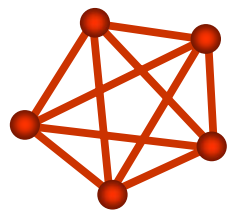
\includegraphics[width=0.4\linewidth]{imgs/lecture11/11.1 non-planar.png}
        \caption{}
        \label{fig:11.1a}
    \end{subfigure}
    \hfill
    \begin{subfigure}[b]{0.45\textwidth}
        \centering
        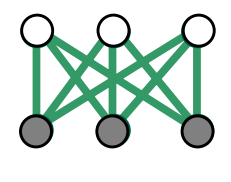
\includegraphics[width=0.4\linewidth]{imgs/lecture11/11.2 non-planar.png}
        \caption{}
        \label{fig:11.1b}
    \end{subfigure}

    \caption{Non-planar drawings}
    \label{fig:11.1}
\end{figure}

The two minimal non-planar graphs: there are two specific structures that make a graph non-planar. Fig \ref{fig:11.1a} is a complete graph with 5 vertices where every vertex is connected to every other vertex. Fig \ref{fig:11.1b} is a complete bipartite graph where two sets of three vertices are connected to each other, also known as the "utility graph"

\subsubsection{The subdivision rule}
A graph does not have to be exactly one of the two drawings in fig. \ref{fig:11.1} to be non-planar; it only needs to contain a subdivision of one of them. A subdivision occurs when new vertices are inserted along the edges of the original structure.